\appendix
 
\chapter{Presupuesto y Planificación}

\section{Presupuesto}

El presupuesto del trabajo se puede separar en dos partes: recursos humanos y amortización de los equipos utilizados.

En cuanto a los recursos humanos empleados, se ha tenido una dedicación por parte del alumno de unas 400 horas, lo que se corresponde dentro del número de horas de dedicación esperadas en la realización de un Trabajo fin de Máster (12 ECTS). Un salario mensual de ayudante investigador a jornada completa en la universidad, es de unos 1250 euros, lo que se traduce en un coste de unos 8,33 euros la hora. El salario del tutor se ha extraído del portal de transparencia de la UPM. La dedicación del tutor ha sido de unas 30 horas de implicación en el trabajo.

\begin{figure}[htb!]
		\centering
		\begin{tabular}{|l|r|r|r|}
		\hline
		%\textbf{Recursos humanos} &Coste unitario [EUR] &Unidades&Total [EUR]\\
		
		\textbf{Recursos humanos} & Horas &Coste Horario [EUR]&Total [EUR]\\
		\hline
		
		Alumno & 400 & 8.33 &  3332 \\
		Tutor & 30& 33.72 & 1011.6 \\
		\hline
		\textbf{Total} & &  & \textbf{4343.6}\\
		\hline
		\end{tabular}\\
	
\end{figure}


En cuanto a la amortización del equipo, se ha empleado un ordenador para el desarrollo del software y para la realización de los experimentos. Se ha considerado una amortización lineal del 10 \% de la vida útil (4 años).

\begin{figure}[htb!]
	\centering
	\begin{tabular}{|l|r|r|r|}
		\hline
		\textbf{Equipo} & Precio &Coste Amortización(10\%)\\
		\hline
		Pc sobremesa & 1980 & 198\\
		\hline
		\textbf{Total} & & \textbf{198}\\
		\hline
\end{tabular}\\
\end{figure}

Con lo que el coste total del proyecto ha sido:

\begin{figure}[htb!]
	\centering
	\begin{tabular}{|l|r|r|r|}
		\hline
		\textbf{Concepto} &Total [EUR]\\
		\hline
		Recursos humanos & 4343.6\\
		Amortización del equipo & 198\\
		
		\hline
		\textbf{Total}   & \textbf{4541.6}\\
		\hline
	\end{tabular}\\
\end{figure}




\newpage
\section{Planificación}
La realización de este trabajo ha empleado un ritmo continuo de horas de trabajo desde su comienzo, a comienzos de abril. La dedicación media invertida en el desarrolo del trabajo ha sido de unas 35 horas semanales, durante un periodo de unos 3 meses, lo que da un total de unas 400 horas. El trabajo se ha realizado dentro del grupo de investigación CVAR (\textit{Computer Vision and Aerial Robotics}) del departamento de Electrónica Automática e Informática industrial de la Escuela Técnica Superior de Ingenieros Industriales (ETSII) perteneciente a la Universidad Politécnica de Madrid (UPM).

En cuanto a la distribución del trabajo en este tiempo, el trabajo comenzó a realizarse a finales de abril de 2020, durante el primer mes se realizó el curso sobre robótica aérea de UPenn, en la plataforma \textit{online} Coursera. La duración del curso se extendió hasta finales de abril. En mayo el trabajo se focalizó en el desarrollo de la arquitectura que se emplearía posteriormente, así como en el estudio del arte de los diferentes algoritmos de control y métodos de generación de trayectorias relevantes en el campo a estudiar. En junio y julio, se realizaron las implementaciones de los distintos algoritmos y se realizaron los primeros experimentos. Finalmente se ha redactado la memoria del proyecto en el mes de Septiembre. Se ha realizado un diagrama GANTT (\cref{gantt}) en el que se ha detallado más en profundidad la distribución temporal de las tareas. Asimismo, se ha esquematizado la organización del proyecto en un diagrama EDP 

\vspace{0.5cm}
\begin{figure}[htb!]
	\centering
	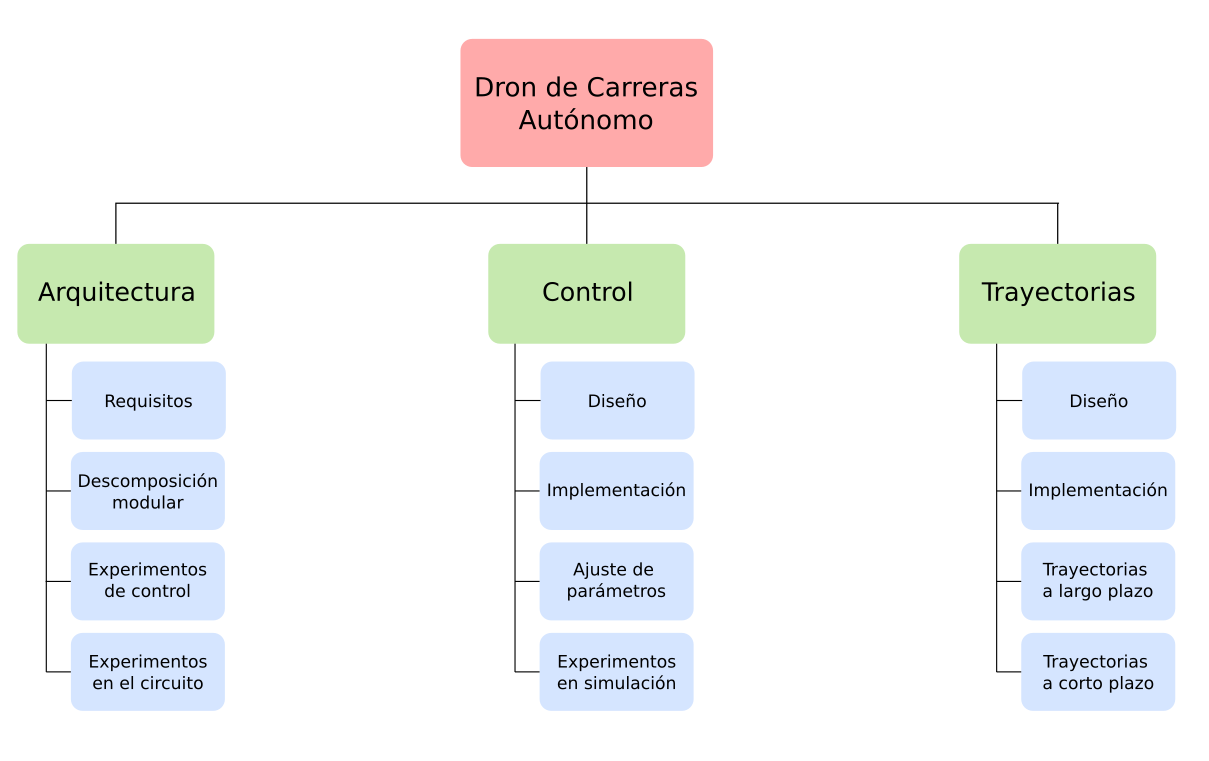
\includegraphics[width=0.85\textwidth]{imagenes/EDP}
	\caption{Diagrama EDP}
	\label{edp}
\end{figure}

\newpage

\textcolor{white}{aligment}
\begin{figure}[htb!]
	\centering
	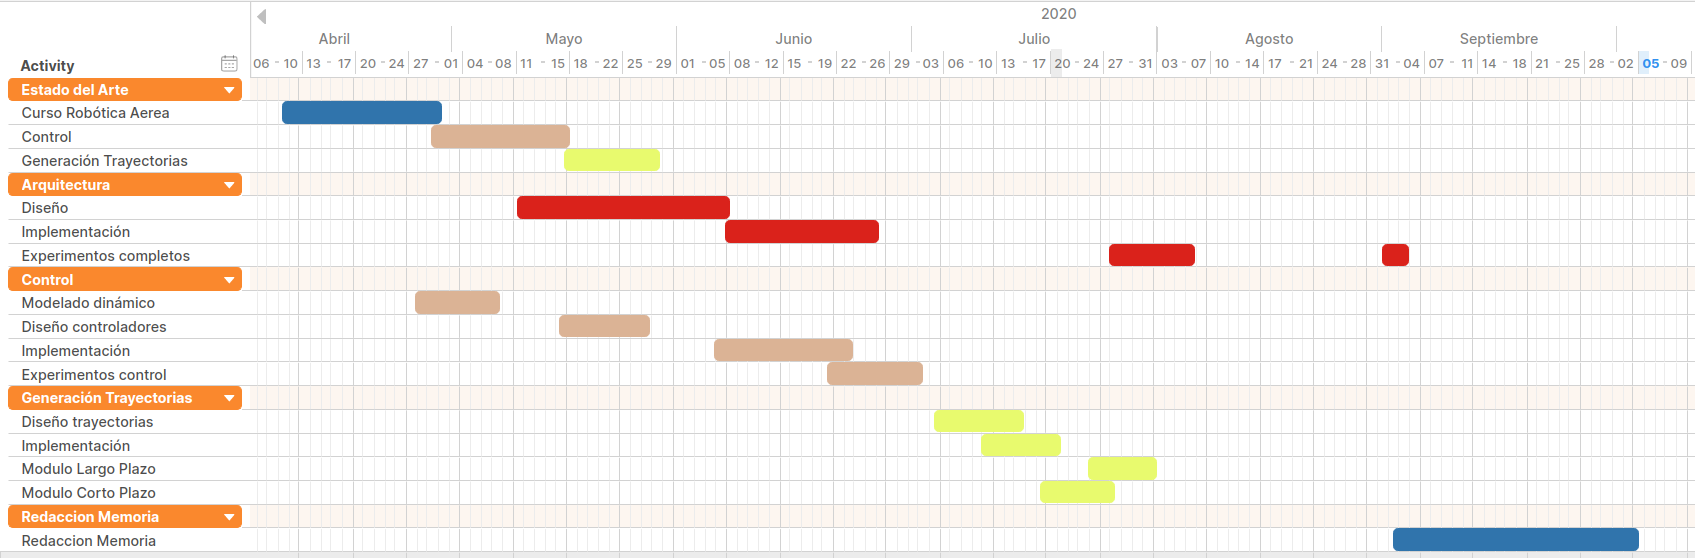
\includegraphics[angle=90,width =0.45\textwidth]{imagenes/gantt}
	\caption{Diagrama Gantt}
	\label{gantt}
\end{figure}

